\usetikzlibrary{graphs,rdf}
\tikzset{
dfa/.style = { semithick, > = To [sep] },
nfa/.style = { semithick, > = To [sep] },
state/.style = { circle, draw, minimum size = 1cm },
final/.style = { double },
initial/.style = { draw = red }, % to keep things simple
transition/.style = { edge label = {$#1$} }
}
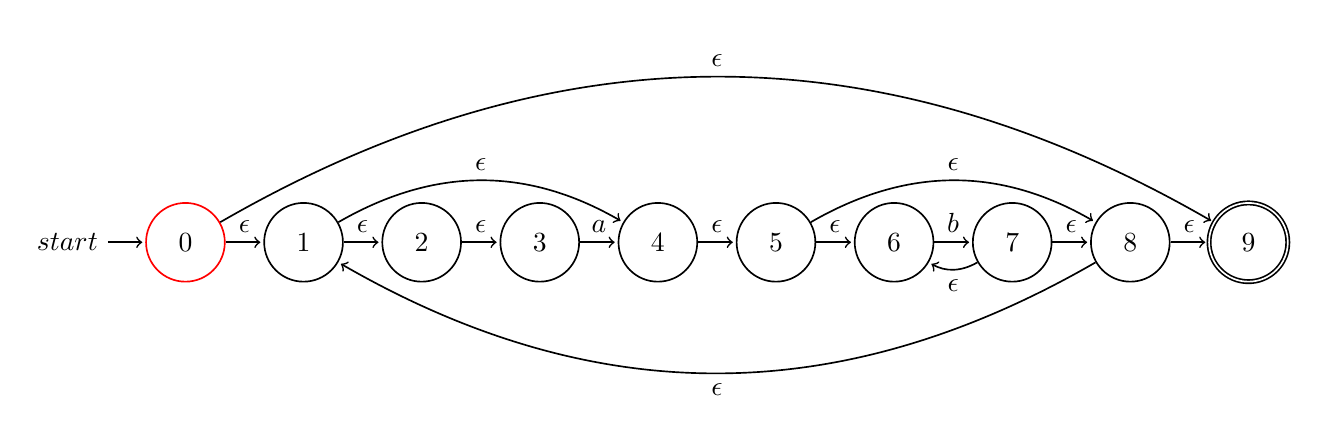
\begin{tikzpicture}[nfa]
	\graph [math nodes, grow right = 1.5cm]{
		start -> 
		0[state,initial] ->[transition=\epsilon]
		1[state] ->[transition=\epsilon]
		2[state] ->[transition=\epsilon]
		3[state] -> [transition=a] 4[state] ->[transition=\epsilon]
		5[state] -> [transition=\epsilon]
		6[state] -> [transition=b] 7[state] ->[transition=\epsilon]
		8[state] ->[transition=\epsilon] 9[final,state];
		1 -> [transition=\epsilon,bend left] 4;
		5 -> [transition=\epsilon,bend left] 8;
		7 -> [transition=\epsilon,bend left] 6;
		8 -> [transition=\epsilon,bend left] 1;
		0 -> [transition=\epsilon,bend left] 9;
	};
\end{tikzpicture}
